\documentclass[aspectratio=169, table]{beamer}

\usepackage{colortbl}
\usepackage{xcolor}
\usepackage{listings}
\usepackage{tikz}
\usepackage{pgfplots}
\usepgfplotslibrary{polar}
\usetikzlibrary{arrows.meta, positioning, calc}

\usetheme{Pradita}


\lstdefinelanguage{bash} {
keywords={},
basicstyle=\ttfamily\small,
keywordstyle=\color{blue}\bfseries,
ndkeywords={iex},
ndkeywordstyle=\color{purple}\bfseries,
sensitive=true,
commentstyle=\color{gray},
stringstyle=\color{red},
numbers=left,
numberstyle=\tiny\color{gray},
breaklines=true,
frame=lines,
backgroundcolor=\color{lightgray!10},
tabsize=2,
comment=[l]{\#},
morecomment=[s]{/*}{*/},
commentstyle=\color{gray}\ttfamily,
stringstyle=\color{purple}\ttfamily,
showstringspaces=false
}

\subtitle{The 2025 10th International STEM Education\\conference (iSTEM-Ed 2025)}

\title{\LARGE Deriving IT Strategies from  \\
Times Higher Education Ranking\\
\vspace{7pt}}

\date[Serial]{Pattaya, Thailand, 30 July-1 August 2025}
\author{\textbf{Alfa Yohannis, Alexander Waworuntu, Master Siregar}}
\begin{document}

\frame{\titlepage}


\begin{frame}[fragile]
\frametitle{Contents}
\vspace{20pt}
\begin{columns}[t]
	\column{0.5\textwidth}
	\tableofcontents[sections={1-8}]
	
	\column{0.5\textwidth}
	\tableofcontents[sections={9-15}]
\end{columns}
\end{frame}

%\begin{frame}{\hfill}
%	\centering
%	\Huge{\textbf{How can data be used to create real strategic, tactical, and operational values?}}
%\end{frame}


\section{Motivation}
\begin{frame}
	\vspace{20pt}
	\frametitle{Motivation}
	\begin{itemize}
		\item \textbf{Digital Shift.} Digital transformation is reshaping Higher Education, demanding agile and data-driven IT strategies.
		\item \textbf{Ranking Impact.} Times Higher Education (THE) rankings influence institutional reputation, funding, and policy.
		\item \textbf{Key Metrics.} THE metrics reflect performance in teaching, research, citations, and international outlook.
		\item \textbf{Strategic Gap.} Universities often lack clear guidance on aligning IT investments with these metrics.
		\item \textbf{Research Aim.} This study explores whether correlations among THE variables can reveal actionable insights for designing impactful IT strategies.
	\end{itemize}
\end{frame}



\section{Objective and Contribution}
\begin{frame}
	\vspace{20pt}
	\frametitle{Objective \& Contribution}
	\begin{itemize}
		\item \textbf{Objective.} Identify the most influential THE ranking variables and derive data-driven IT strategies that universities can adopt to improve performance and competitiveness.
		\item \textbf{Contribution.}
		\begin{itemize}
			\item Longitudinal dataset spanning 11 years (2013–2023) with more than 700 universities analysed.
			\item Application of Spearman’s rank correlation to uncover robust relationships among ranking metrics.
			\item Practical IT strategy recommendations grounded in statistical evidence to support teaching, research, citations, and global engagement.
		\end{itemize}
	\end{itemize}
\end{frame}


\section{Literature Landscape}
\begin{frame}
	\vspace{20pt}
	\frametitle{Literature Landscape}
	\begin{itemize}
		\item \textbf{Existing Focus.} Prior research addresses IT strategy frameworks such as COBIT and enterprise architecture, alignment between IT and institutional goals, and the influence of global rankings in higher education.
		\item \textbf{Research Gap.} Few studies directly link Times Higher Education (THE) indicators—like research, teaching, or international outlook—to specific IT strategy formulation.
		\item \textbf{This Study.} Bridges that gap by analysing THE variables to inform evidence-based IT strategy development.
	\end{itemize}
\end{frame}


\section{Methodology}
\begin{frame}
	\vspace{20pt}
	\frametitle{Methodology Overview}
	\begin{itemize}
		\item \textbf{Data Collection.} Combined 11 years of THE ranking data (2013–2023) via web scraping, covering 711 universities.
		\item \textbf{Analytical Approach.} Used Spearman’s rank correlation to assess relationships without assuming normal distribution.
		\item \textbf{Tooling.} Python scripts with the related libraries (e.g., pandas, matplotlib,etc.)were used for scraping, processing, and analysing.
		\item \textbf{Observed Variables.} Eleven key indicators from THE were analysed: Overall Score (OS), Rank (R), Research Score (RS), Teaching Score (TS), Citations Score (CS), International Outlook (IO), International Students (IS), Industry Income (II), Student-to-Staff Ratio (SSR), Number of Students (NS), and Year (Y).
		
	\end{itemize}
\end{frame}

\begin{frame}{Overall Correlations Result}
	\vspace{10pt}
	\centering
	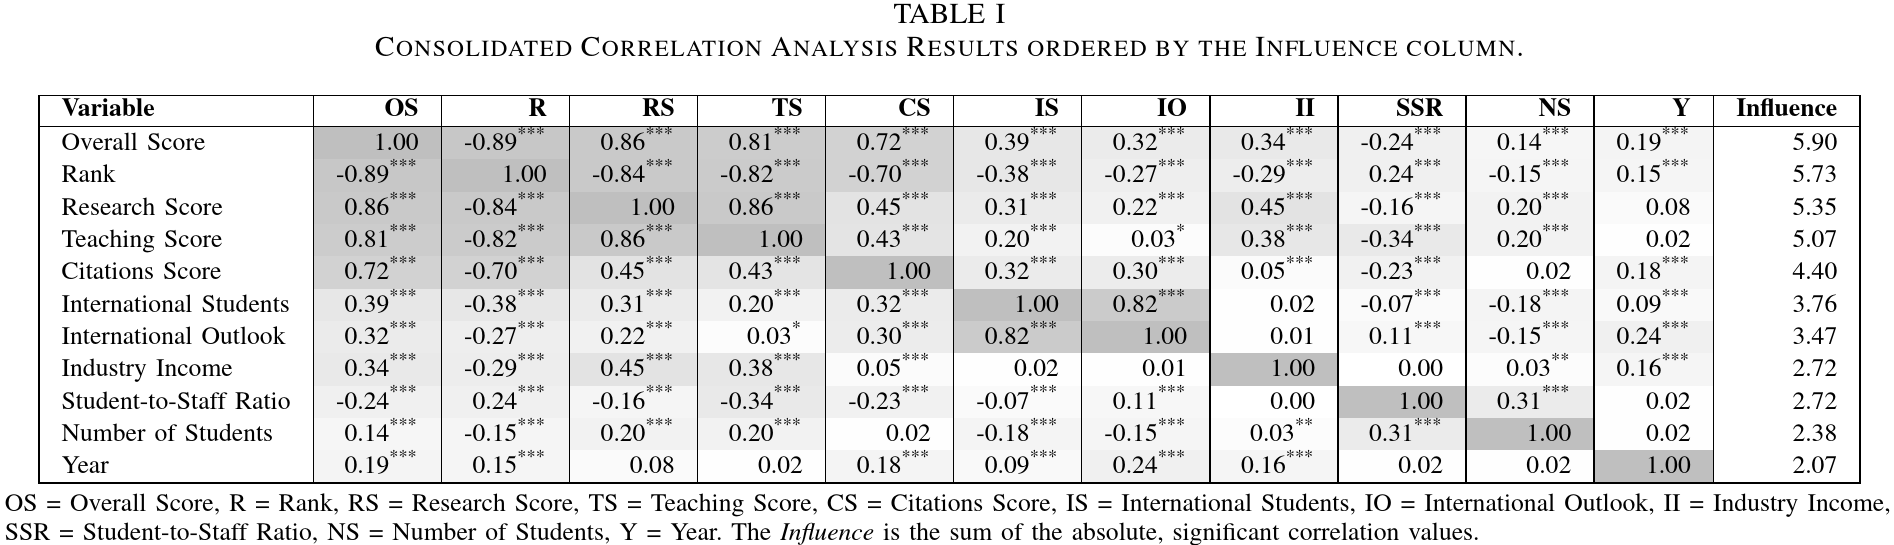
\includegraphics[width=1.03\linewidth]{figures/table1.png}
\end{frame}

\begin{frame}
	\vspace{20pt}
	\frametitle{Top Correlation Findings}
	\begin{itemize}
		\item \textbf{Rank} \textbf{strongly improves} with: (negative correlations indicate better rank -- lower value -- with higher performance)
		\begin{itemize}
			\item \textbf{Overall Score:} $r = -0.89$
			\item \textbf{Research Score:} $r = -0.84$
			\item \textbf{Teaching Score:} $r = -0.82$
		\end{itemize}
		\item \textbf{Citations Score:} $r = -0.70$ highlights the role of research visibility.
		\item \textbf{Internationalisation metrics} like International Students ($r = -0.38$) and Outlook ($r = -0.27$) also help but are secondary.
		\item \textbf{Implication.} Universities aiming to rise in rank should prioritise improving research quality, teaching effectiveness, and publication impact, while building global partnerships as supportive strategies.
		
	\end{itemize}
\end{frame}



\section{Influence Summary}
\begin{frame}
	\vspace{20pt}
	\frametitle{Total Influence Summary}
	\begin{itemize}
		\item \textbf{Top 5 most influential variables} based on the sum of absolute significant correlations:
		\begin{itemize}
			\item Overall Score (OS): 5.90
			\item Rank (R): 5.73
			\item Research Score (RS): 5.35
			\item Teaching Score (TS): 5.07
			\item Citations Score (CS): 4.40
		\end{itemize}
		\item \textbf{Moderate contributors} include International Students (IS: 3.76), International Outlook (IO: 3.47), and Industry Income (II: 2.72).
		\item \textbf{Implication:} Institutional strategies should prioritise research, teaching, and publication impact while strengthening global visibility and partnerships for long-term ranking improvements.
	\end{itemize}
\end{frame}


\section{Individual Case Example: X University}

\begin{frame}{Individual Case Example: X University}
	\vspace{10pt}
	\centering
	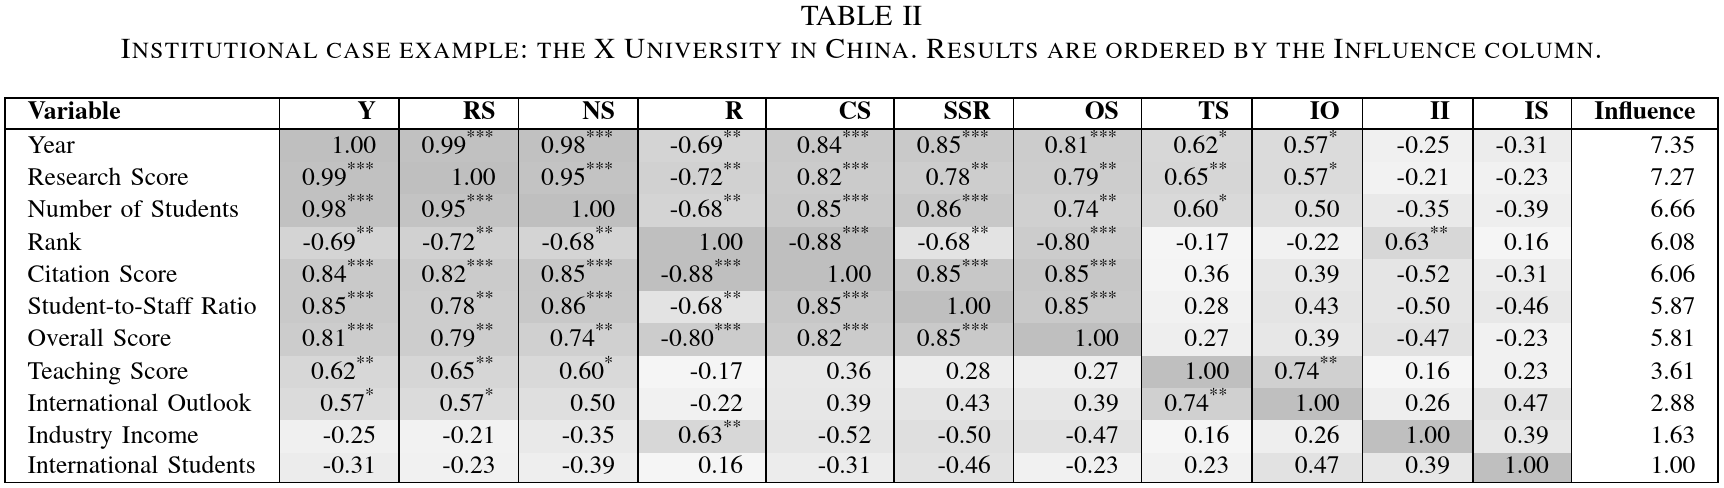
\includegraphics[width=1.03\linewidth]{figures/table2.png}
\end{frame}

\begin{frame}
	\vspace{20pt}
	\frametitle{Case Example: X University}
	\begin{itemize}
		\item \textbf{Most Influential Variables.} Year (7.35), Research Score (7.27), and Number of Students (6.66) had the strongest influence across metrics.
		\item \textbf{Secondary Influencers.} Citation Score (6.06), Rank (6.08), and Student-to-Staff Ratio (5.87) also played significant roles in shaping institutional profile.
		\item \textbf{Less Influence.} Teaching (3.61), International Outlook (2.88), Industry Income (1.63), and International Students (1.00).
		\item \textbf{Implication.} The institutional is progressing well every year and appears research-driven and scale-oriented, with less emphasis on globalisation (local-oriented?) and financial diversification (government support?).
	\end{itemize}
\end{frame}


\section{IT Strategy Focus}
\begin{frame}
	\vspace{20pt}
	\frametitle{Focus Areas: Why These Matter}
	\begin{itemize}
		\item \textbf{Research (RS, 5.35)}: Strongly influences both teaching and overall scores, and is a consistent driver of academic reputation.
		
		\item \textbf{Teaching (TS, 5.07)}: Closely intertwined with research and rank, reflecting its role in both educational quality and institutional prestige.
		
		\item \textbf{Citations (CS, 4.40)}: Directly associated with research strength and international recognition, making it a vital performance indicator.
		
		\item \textbf{Internationalisation (IS, 3.76; IO, 3.47)}: Enhances global visibility and ranking metrics; positively correlates with teaching, citations, and research.
		
		\item \textbf{Industry Income (II, 2.72)}: Provides applied value from research outputs and builds external relevance.
		
		\item \textbf{Efficiency Metrics (SSR, 2.72; NS, 2.38)}: Reflect institutional scale and resource allocation, affecting perceptions of academic support and capacity.
	\end{itemize}
\end{frame}



\section{Recommendations (1/2)}
\begin{frame}
	\vspace{20pt}
	\frametitle{Top IT Strategy Recommendations (1/2)}
	\begin{itemize}
		\item \textbf{Learning Experience Platform.} Enhance teaching (TS) and research (RS) through adaptive content and analytics.
		\item \textbf{Research Info Management System (RIMS).} Streamline research workflows and open-access publishing to improve RS.
		\item \textbf{Bibliometric Dashboards.} Track citations and journal impact to boost citation scores (CS).
		\item \textbf{Global Engagement Portal.} Support joint degree programmes and international admissions to strengthen International Outlook (IO) and International Students (IS) metrics.
		
		\item \textbf{Industry Partner Tracker.} Publish and monitor patents, research, and projects to grow industry income (II).
	\end{itemize}
\end{frame}


\section{Recommendations (2/2)}
\begin{frame}
	\vspace{20pt}
	\frametitle{Top IT Strategy Recommendations (2/2)}
	\begin{itemize}
		\item \textbf{Predictive ERP + Timetabling.} Forecast staffing needs and optimise class sizes to improve the student-to-staff ratio (SSR).
		\item \textbf{Strategic KPI Dashboard.} Track progress and align IT projects with THE ranking indicators or other contextual indicators.
		\item \textbf{Digital Roadmap.} Maintain a long-term transformation plan to adapt to the gradual, yearly shifts (Y).
		\item \textbf{AI Segmentation for International Students.} Personalise support and boost global engagement (IS).
		\item \textbf{Unified Analytics Platform.} Combine institutional data to drive coordinated improvements across THE dimensions.
	\end{itemize}
\end{frame}



\section{Implementation Guidance}
\begin{frame}
	\vspace{20pt}
	\frametitle{Implementation Considerations}
	\begin{itemize}
		\item \textbf{Institutional Fit.} Strategies should align with the university’s digital maturity, policies, and organisational readiness.
		\item \textbf{Phased Rollout.} Implement in modular stages to minimise disruption and manage risk.
		\item \textbf{Agile Governance.} Use adaptive decision-making structures to respond to changes in technology and ranking indicators.
		\item \textbf{Contextual Customisation.} Tailor each solution to local needs, infrastructure, and stakeholder expectations to ensure relevance and sustainability.
	\end{itemize}
\end{frame}

\section{Study Limitations}
\begin{frame}
	\vspace{20pt}
	\frametitle{Limitations}
	\begin{itemize}
		\item \textbf{Correlation Does Not Imply Causation.} The analysis identifies associations, but not causal relationships.
		\item \textbf{Potential Confounding Factors.} Other unmeasured variables may influence the observed correlations.
		\item \textbf{Need for Further Research.} Longitudinal or experimental designs are required to validate directional effects of the strategies.
		\item \textbf{Limited Data Scope.} The study is based on data from 711 universities over 11 years, which may not capture all global contexts.
		\item \textbf{Ranking System Bias.} Results are based solely on Times Higher Education; other global ranking systems should be explored for broader validation.
	\end{itemize}
\end{frame}


\section{Conclusion}
\begin{frame}
	\vspace{20pt}
	\frametitle{Conclusion}
	\begin{itemize}
		\item \textbf{Core Influence.} Research and teaching scores have the strongest impact on institutional rank, followed by citations and internationalisation.
		\item \textbf{Data-Driven Strategy.} Times Higher Education indicators provide a solid foundation for shaping evidence-based IT strategies.
		\item \textbf{Priority Areas.} Improving research performance, citation impact, global engagement, and industry collaboration can enhance overall institutional outcomes.
		\item \textbf{Strategic Value.} Aligning IT investments with influential ranking metrics supports long-term competitiveness and academic excellence in higher education.
	\end{itemize}
\end{frame}





%\begin{frame}{Orange Workflow for Loan Approval Model}
%	\vspace{10pt}
%	\centering
%	\includegraphics[width=\linewidth]{../../figures/decision_tree_pipeline.png}
%\end{frame}



\end{document}
